\chapter{Replication}

\begin{definition}
   [Replication]
   Replication is the process of sharing information so as to ensure consistency between redundant resources, such as software or hardware components, to improve reliability, fault-tolerance, or accessibility.

\end{definition}

The aims of replication are reducing latency, increasing availability, and scaling read throughput.
However replication clearly poses some potential problems when handling changes to replicated data.
{The possible approaches to replication are:\ns
\begin{itemize}
   \item single-leader
   \item multi-leader
   \item leaderless replication
\end{itemize}}

\section{Leaders and followers}
Each node may store a copy of the database, in this case it is called a \textbf{replica}, so, ensuring consistency among replicas is crucial.



With leader based replication, one replica is designated as the \textit{leader} who receives write requests by clients, and is responsible for writing new data to its local storage.
Later on, Followers update their local copy based on the leader's
replication log.

\subsection{Synchronous vs Asynchronous Replication}
\begin{itemize}
   \item \textbf{Synchronous} - The \ul{leader waits for the followers} to acknowledge the write before acknowledging the write itself.
   \begin{itemize}
      \item Ensures that followers have an up-to-date copy of the data.
      \item The disadvantage is that the system may become unavailable if a follower is slow to respond.
   \end{itemize}
   \item \textbf{Asynchronous} - The \ul{leader does \textbf{not} wait for the followers} to acknowledge the write before acknowledging the write itself.
   \begin{itemize}
      \item Follower may fall behind the leader.
      \item The advantage is that the system continues processing even if a follower is slow to respond.
      \item The disadvantage is that the system may lose data if the leader fails before the followers have caught up, so there's the need for methods to ensure data integrity.
   \end{itemize}
   \item \textbf{Semi-synchronous} - The \ul{leader waits for a \textbf{quorum} of followers} (at least one follower, typically always the same and placed in another location) to acknowledge the write before acknowledging the write itself.
   \begin{itemize}
      \item Ensures that at least one follower has an up-to-date copy of the data.
      \item Typically there is \ul{only one node fully synchronous}, while others are asynchronous, and it is \ul{placed far away from the leader}.
   \end{itemize}
\end{itemize}

\section{Failure}
\begin{itemize}
   \item \textbf{Node} failures - Nodes can fail due to faults or planned maintenance. The goal is to minimize impact and keep the system running.
   \item \textbf{Follower} failure: Catch up recovery - Followers keep a log of data changes, but can catch up with the leader if they fall behind.
   \item \textbf{Leader} failure: Failover - Failover process involves promoting ---hence reconfiguring--- a follower to leader. Failover can be manual or automatic
   \item Challenges in \textbf{Failover} - Asynchronous replication may lead to data loss, as stated before.
\end{itemize}

\subsection{Implementing Replication Logs}
\begin{itemize}
   \item \textbf{Statement-based} replication - Replicate SQL write requests statements from the leader to the followers.
   \note{We cannot ensure a fully consistent system, due to issues with non-deterministic functions, autoincrementing columns, and side effects.\\
   This was used in VoltDB and MySQL before version 5.1.}
   \item \textbf{Write-ahead log (WAL)} shipping - Replicate the log of changes to the database from the leader to the followers.
   \note{Still some problems here, because we assume that the leader and the followers are using the same database engine, same architecture an so on, so that the log is the same.}
   \item \textbf{Logical log} replication - Replicate a logical representation of changes to the database from the leader to the followers.
   \note{This is advantageous and flexible, but it is dischouraged by the fact that some expertise and coding are required. Instead, with the first two approaches there is no need to modify the database in any way.}
   \item \textbf{Trigger-based} replication - Replicate changes to the database by using triggers.
\end{itemize}


\section{Eventual Consistency}
The eventual consistency model implies a temporary state where the followers lag behind the leader, but eventually they will catch up. 
Hence there is some ``replication-lag'' \dots

However, many modern applications require heavy reading workload, but light writing workload, so eventual consistency is a good trade-off.
Besides it is possible to increase capacity for read- only requests by adding more followers. Removes load from the leader. Allows read requests to be served by nearby replicas 

\subsection{Read-after-write consistency}
\begin{paracol}{2}
   \begin{figure}[htbp]
      \centering
      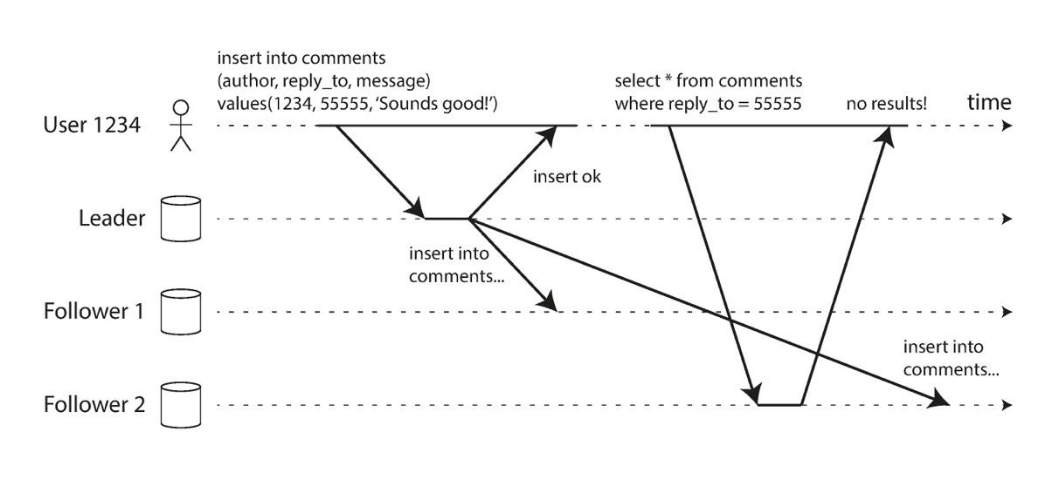
\includegraphics[width=0.95\columnwidth]{images/10/readafterwrite.png}
      \caption{Read-after-write consistency time schema}
      \label{fig:10/readafterwrite}
   \end{figure}


   \switchcolumn
   \colfill
   In asynchronous replication it is not trivial to ensure \textit{read-your-write} consistency, i.e. if a client writes a value to the leader, it should be able to read it.
   In other words, a user may think their data is lost, because they cannot see it, but it is actually there, just not yet replicated to the follower.
   
   \textit{Read-after-write} consistency guarantees that \ul{users see their own updates, but not necessarily the updates of others.}
   It may be implemented by reading user-modified data from the leader.
   \colfill
\end{paracol}


\subsection{Monotonic Reads}

\begin{paracol}{2}
   \begin{figure}[htbp]
      \centering
      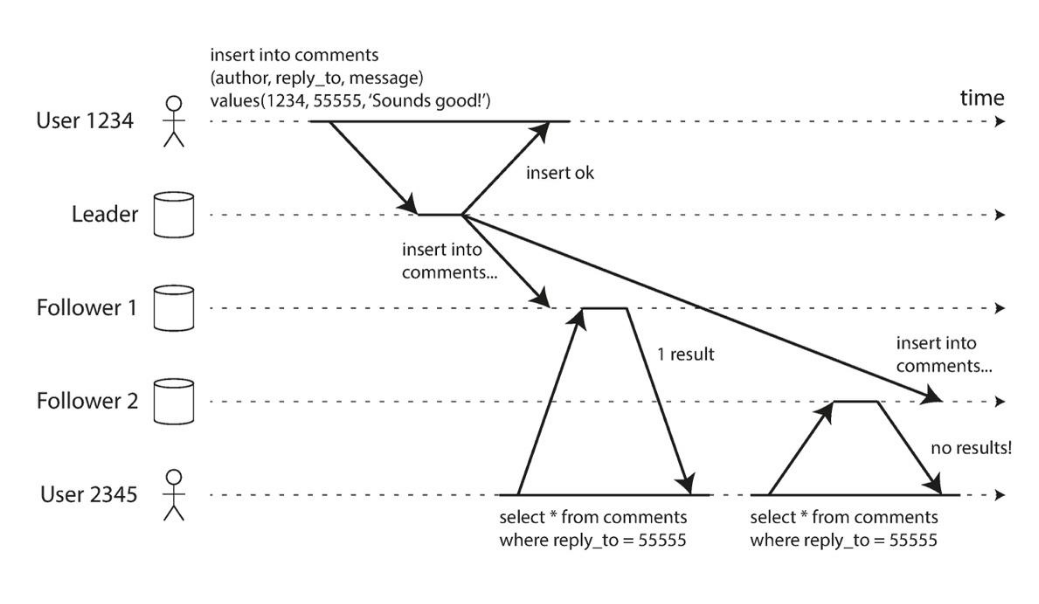
\includegraphics[width=0.95\columnwidth]{images/10/monotonic.png}
      \caption{Monotonic reads time schema}
      \label{fig:10/monotonic}
   \end{figure}
   
   
   \switchcolumn
   \colfill
   \textit{Monotonic reads} consistency guarantees that if a user has read the value of a key, it will not read an older value of the same key in the future.
   It is stronger than eventual consistency, but weaker than strong consistency.
   
   In asynchronous replication may see data moving backward in time when reading from different replicas with varying lag.\\
   Monotonic reads can be achieved by ensuring that reads are always performed on the same replica.
   \colfill
\end{paracol}


\newpage
\subsection{Consistent Prefix Reads w/different DBs}

\begin{paracol}{2}
   \begin{figure}[htbp]
      \centering
      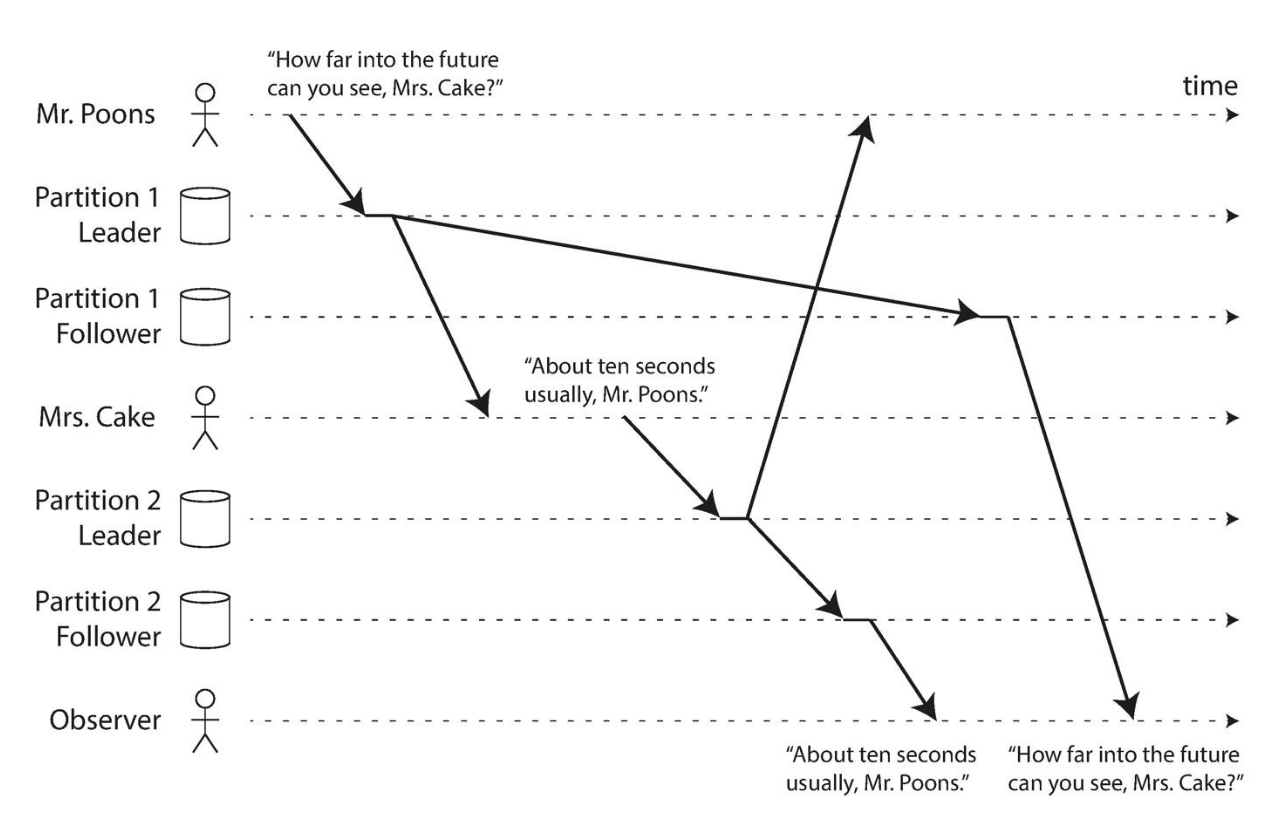
\includegraphics[width=0.95\columnwidth]{images/10/consistentprefix.png}
      \caption{Consistent prefix reads with different DBs}
      \label{fig:10/consistentprefixs}
   \end{figure}

   \switchcolumn
   \colfill
   \textit{Consistent prefix reads} consistency guarantees that if a sequence of writes happens in a certain order, then a read will see those writes in the same order.
   
   Suppose that $A$ asks $B$ something, and $C$ is listening, but hears first the answers and later the question: weird, ain't it?\\
   This may happen due to replication lag. We want to prevent casuality violations.
   \colfill
\end{paracol}



\section{Multi-Leader Replication}
With a single-leader configuration, the leader is a bottleneck, and if it fails, the system elects a new leader (perhaps there may be a small downtime).

With multi-leader replication, there are multiple leaders, and each leader can accept writes. This is useful for geographically distributed systems, where each region has its own leader.

\subsection{Collaborative Editing}
\ul{Real-time collaborative editing is a use case for multi-leader replication.}\\
Changes are instantly appied to the user's local replica and then asynchronously replicated to the server and other users.

Application must obtain a lock on the document before editing, as with single leader replication with transactions (?).\\
The unit of change may be small, as a single keystroke.\nl

When two users edit the same part of the document, they get local updates, but when the system asynchronously synchronizes the replicas, a conflict occurs and needs resolution.\\
With single-leader replication, the second writer blocks or aborts if first write is incomplete, having the user to retry the input.\\
With multi-leader replication, the system must resolve the conflict, and the user must be notified of the resolution.

\subsection{Conflict Avoidance}
\labelitemize{Strategies}{
   \begin{itemize}
      \item Routing writes towards the same leader prevents conflicts.
      \item Routing user requests towards the same datacenter allows to use only the leader of that datacenter; furthermore, geographical locality may be applied, to serve a user with the closest datacenter.
   \end{itemize}
}

% // Prof SKIPPING a few slides starting from "consistent and converging to a state"


\subsection{Topologies}
\begin{itemize}
   \item \textbf{Circular} - each node receives writes and forwards writes
   \item \textbf{Star topology} - root node forwards writes to all other nodes 
   \item \textbf{All-to-all} - every leader sends writes to every other leader
\end{itemize}

Note that this is not hardware (neither virtual) network, but a logical network of replication, made up by how we manage the information flow.

In whatever topology it is important to \textbf{monitor staleness}, which is monitoring obsolete replicas, i.e. how far behind a follower is from the leader.

\subsection{Concurrent Writes}
Several clients can write to the same key simultaneously, and the order of writes may differ on different leaders. So\dots ``who wins?''

\begin{itemize}
   \item \textbf{Last write wins} - The last write is the one that is kept.
   \item \textbf{Most recent timestamp wins} - The write with the most recent timestamp is the one that is kept.
   \item \textbf{Merge values} - The values are merged together, based on a \textit{happens-before} relationship.
\end{itemize}

However, especially for geographically spread databases, it is not trivial to determine the most recent timestamp, because clocks may be unsynchronized, and also the network latency may vary. Remember also that the light speed is finite, so it takes time for a signal to travel from one point to another.\\
For this reason the \textit{happens-before} relationship is used, which is a partial order on events, which reflects the order in which events have occurred.